\documentclass[11pt]{article}

\usepackage[T1]{fontenc}
\usepackage[utf8]{inputenc}
\usepackage{lmodern}
\usepackage{microtype}
\usepackage[margin=1in]{geometry}
\usepackage{amsmath}
\usepackage{booktabs}
\usepackage{tabularx}
\usepackage{array}
\usepackage{enumitem}
\usepackage{xcolor}
\usepackage{listings}
\usepackage{tikz}
\usetikzlibrary{arrows.meta,positioning,shapes.geometric,calc}
\usepackage[numbers,sort&compress]{natbib}
\usepackage[hidelinks]{hyperref}
\usepackage{url}

\setlist{itemsep=2pt,topsep=4pt}
\newcolumntype{L}{>{\raggedright\arraybackslash}X}

\lstset{
  language=Python,
  basicstyle=\ttfamily\footnotesize,
  keywordstyle=\bfseries,
  commentstyle=\itshape\color{black!60},
  stringstyle=\color{black!75},
  frame=single,
  rulecolor=\color{black!30},
  columns=fullflexible,
  keepspaces=true,
  showstringspaces=false,
  breaklines=true,
  xleftmargin=4pt,
  xrightmargin=4pt,
}

\newcommand{\toolname}{Code2Test}
\newcommand{\code}[1]{\texttt{#1}}

% Measured results, generated from research/data by research/scripts/collect_results.py
% Generated by research/scripts/collect_results.py from research/data. Do not edit.
\newcommand{\InflectionFlashComponents}{13}
\newcommand{\InflectionFlashWithTests}{13}
\newcommand{\InflectionFlashAcceptance}{100\%}
\newcommand{\InflectionFlashGenerated}{205}
\newcommand{\InflectionFlashFirstPassed}{196}
\newcommand{\InflectionFlashFirstRate}{96\%}
\newcommand{\InflectionFlashKept}{205}
\newcommand{\InflectionFlashXfail}{0}
\newcommand{\InflectionFlashDropped}{0}
\newcommand{\InflectionFlashRepairs}{8}
\newcommand{\InflectionFlashCasesPassed}{408}
\newcommand{\InflectionFlashCasesTotal}{408}
\newcommand{\InflectionFlashCasesSkipped}{0}
\newcommand{\InflectionFlashSeconds}{193}
\newcommand{\InflectionFlashMutants}{80}
\newcommand{\InflectionFlashKilled}{47}
\newcommand{\InflectionFlashMutationScore}{59\%}
\newcommand{\InflectionFlashKilledOwn}{40}
\newcommand{\InflectionFlashOwnScore}{50\%}
\newcommand{\InflectionFlashDiagAccuracy}{97\%}
\newcommand{\InflectionFlashDiagCorrect}{29}
\newcommand{\InflectionFlashDiagCases}{30}
\newcommand{\InflectionFlashCodeBugCorrect}{14}
\newcommand{\InflectionFlashCodeBugCases}{15}
\newcommand{\InflectionFlashTestWrongCorrect}{15}
\newcommand{\InflectionFlashTestWrongCases}{15}
\newcommand{\InflectionFlashIntentsBelow}{0}
\newcommand{\InflectionFlashIntentsFromModel}{0}
\newcommand{\InflectionFlashSurvivors}{33}
\newcommand{\InflectionFlashStringSurvivors}{8}
\newcommand{\InflectionFlashTopComponent}{\code{\_irregular}}
\newcommand{\InflectionFlashTopMutants}{40}
\newcommand{\InflectionFlashTopKilled}{9}
\newcommand{\InflectionFlashRestMutants}{40}
\newcommand{\InflectionFlashRestKilled}{38}
\newcommand{\InflectionMThreeComponents}{13}
\newcommand{\InflectionMThreeWithTests}{13}
\newcommand{\InflectionMThreeAcceptance}{100\%}
\newcommand{\InflectionMThreeGenerated}{172}
\newcommand{\InflectionMThreeFirstPassed}{147}
\newcommand{\InflectionMThreeFirstRate}{85\%}
\newcommand{\InflectionMThreeKept}{172}
\newcommand{\InflectionMThreeXfail}{0}
\newcommand{\InflectionMThreeDropped}{0}
\newcommand{\InflectionMThreeRepairs}{5}
\newcommand{\InflectionMThreeCasesPassed}{326}
\newcommand{\InflectionMThreeCasesTotal}{326}
\newcommand{\InflectionMThreeCasesSkipped}{0}
\newcommand{\InflectionMThreeSeconds}{407}
\newcommand{\InflectionMThreeMutants}{80}
\newcommand{\InflectionMThreeKilled}{58}
\newcommand{\InflectionMThreeMutationScore}{73\%}
\newcommand{\InflectionMThreeKilledOwn}{52}
\newcommand{\InflectionMThreeOwnScore}{65\%}
\newcommand{\InflectionMThreeDiagAccuracy}{100\%}
\newcommand{\InflectionMThreeDiagCorrect}{30}
\newcommand{\InflectionMThreeDiagCases}{30}
\newcommand{\InflectionMThreeCodeBugCorrect}{15}
\newcommand{\InflectionMThreeCodeBugCases}{15}
\newcommand{\InflectionMThreeTestWrongCorrect}{15}
\newcommand{\InflectionMThreeTestWrongCases}{15}
\newcommand{\InflectionMThreeIntentsBelow}{0}
\newcommand{\InflectionMThreeIntentsFromModel}{0}
\newcommand{\InflectionMThreeSurvivors}{22}
\newcommand{\InflectionMThreeStringSurvivors}{8}
\newcommand{\InflectionMThreeTopComponent}{\code{\_irregular}}
\newcommand{\InflectionMThreeTopMutants}{40}
\newcommand{\InflectionMThreeTopKilled}{18}
\newcommand{\InflectionMThreeRestMutants}{40}
\newcommand{\InflectionMThreeRestKilled}{40}
\newcommand{\TinyDBFlashComponents}{26}
\newcommand{\TinyDBFlashWithTests}{25}
\newcommand{\TinyDBFlashAcceptance}{96\%}
\newcommand{\TinyDBFlashGenerated}{471}
\newcommand{\TinyDBFlashFirstPassed}{411}
\newcommand{\TinyDBFlashFirstRate}{87\%}
\newcommand{\TinyDBFlashKept}{458}
\newcommand{\TinyDBFlashXfail}{0}
\newcommand{\TinyDBFlashDropped}{13}
\newcommand{\TinyDBFlashRepairs}{22}
\newcommand{\TinyDBFlashCasesPassed}{530}
\newcommand{\TinyDBFlashCasesTotal}{531}
\newcommand{\TinyDBFlashCasesSkipped}{1}
\newcommand{\TinyDBFlashSeconds}{314}
\newcommand{\TinyDBFlashMutants}{80}
\newcommand{\TinyDBFlashKilled}{62}
\newcommand{\TinyDBFlashMutationScore}{78\%}
\newcommand{\TinyDBFlashKilledOwn}{61}
\newcommand{\TinyDBFlashOwnScore}{76\%}
\newcommand{\TinyDBFlashDiagAccuracy}{100\%}
\newcommand{\TinyDBFlashDiagCorrect}{30}
\newcommand{\TinyDBFlashDiagCases}{30}
\newcommand{\TinyDBFlashCodeBugCorrect}{15}
\newcommand{\TinyDBFlashCodeBugCases}{15}
\newcommand{\TinyDBFlashTestWrongCorrect}{15}
\newcommand{\TinyDBFlashTestWrongCases}{15}
\newcommand{\TinyDBFlashIntentsBelow}{2}
\newcommand{\TinyDBFlashIntentsFromModel}{2}
\newcommand{\TinyDBFlashSurvivors}{18}
\newcommand{\TinyDBFlashStringSurvivors}{14}
\newcommand{\TinyDBFlashTopComponent}{\code{Table}}
\newcommand{\TinyDBFlashTopMutants}{26}
\newcommand{\TinyDBFlashTopKilled}{21}
\newcommand{\TinyDBFlashRestMutants}{54}
\newcommand{\TinyDBFlashRestKilled}{41}
\newcommand{\TinyDBMThreeComponents}{26}
\newcommand{\TinyDBMThreeWithTests}{25}
\newcommand{\TinyDBMThreeAcceptance}{96\%}
\newcommand{\TinyDBMThreeGenerated}{297}
\newcommand{\TinyDBMThreeFirstPassed}{294}
\newcommand{\TinyDBMThreeFirstRate}{99\%}
\newcommand{\TinyDBMThreeKept}{296}
\newcommand{\TinyDBMThreeXfail}{0}
\newcommand{\TinyDBMThreeDropped}{1}
\newcommand{\TinyDBMThreeRepairs}{4}
\newcommand{\TinyDBMThreeCasesPassed}{432}
\newcommand{\TinyDBMThreeCasesTotal}{432}
\newcommand{\TinyDBMThreeCasesSkipped}{0}
\newcommand{\TinyDBMThreeSeconds}{815}
\newcommand{\TinyDBMThreeMutants}{80}
\newcommand{\TinyDBMThreeKilled}{61}
\newcommand{\TinyDBMThreeMutationScore}{76\%}
\newcommand{\TinyDBMThreeKilledOwn}{61}
\newcommand{\TinyDBMThreeOwnScore}{76\%}
\newcommand{\TinyDBMThreeDiagAccuracy}{100\%}
\newcommand{\TinyDBMThreeDiagCorrect}{30}
\newcommand{\TinyDBMThreeDiagCases}{30}
\newcommand{\TinyDBMThreeCodeBugCorrect}{15}
\newcommand{\TinyDBMThreeCodeBugCases}{15}
\newcommand{\TinyDBMThreeTestWrongCorrect}{15}
\newcommand{\TinyDBMThreeTestWrongCases}{15}
\newcommand{\TinyDBMThreeIntentsBelow}{2}
\newcommand{\TinyDBMThreeIntentsFromModel}{2}
\newcommand{\TinyDBMThreeSurvivors}{19}
\newcommand{\TinyDBMThreeStringSurvivors}{12}
\newcommand{\TinyDBMThreeTopComponent}{\code{Table}}
\newcommand{\TinyDBMThreeTopMutants}{27}
\newcommand{\TinyDBMThreeTopKilled}{14}
\newcommand{\TinyDBMThreeRestMutants}{53}
\newcommand{\TinyDBMThreeRestKilled}{47}
\newcommand{\MinAcceptance}{96\%}
\newcommand{\MaxAcceptance}{100\%}
\newcommand{\MinFirstRate}{85\%}
\newcommand{\MaxFirstRate}{99\%}
\newcommand{\MinMutationScore}{59\%}
\newcommand{\MaxMutationScore}{78\%}
\newcommand{\MinOwnScore}{50\%}
\newcommand{\MaxOwnScore}{76\%}
\newcommand{\MinDiagAccuracy}{97\%}
\newcommand{\MaxDiagAccuracy}{100\%}
\newcommand{\NumRuns}{4}
\newcommand{\InflectionFlashSecondComponents}{13}
\newcommand{\InflectionFlashSecondWithTests}{13}
\newcommand{\InflectionFlashSecondAcceptance}{100\%}
\newcommand{\InflectionFlashSecondGenerated}{230}
\newcommand{\InflectionFlashSecondFirstPassed}{194}
\newcommand{\InflectionFlashSecondFirstRate}{84\%}
\newcommand{\InflectionFlashSecondKept}{230}
\newcommand{\InflectionFlashSecondXfail}{0}
\newcommand{\InflectionFlashSecondDropped}{0}
\newcommand{\InflectionFlashSecondRepairs}{14}
\newcommand{\InflectionFlashSecondCasesPassed}{476}
\newcommand{\InflectionFlashSecondCasesTotal}{476}
\newcommand{\InflectionFlashSecondCasesSkipped}{0}
\newcommand{\InflectionFlashSecondSeconds}{512}
\newcommand{\InflectionFlashSecondMutants}{80}
\newcommand{\InflectionFlashSecondKilled}{48}
\newcommand{\InflectionFlashSecondMutationScore}{60\%}
\newcommand{\InflectionFlashSecondKilledOwn}{42}
\newcommand{\InflectionFlashSecondOwnScore}{53\%}
\newcommand{\InflectionFlashSecondDiagAccuracy}{100\%}
\newcommand{\InflectionFlashSecondDiagCorrect}{30}
\newcommand{\InflectionFlashSecondDiagCases}{30}
\newcommand{\InflectionFlashSecondCodeBugCorrect}{15}
\newcommand{\InflectionFlashSecondCodeBugCases}{15}
\newcommand{\InflectionFlashSecondTestWrongCorrect}{15}
\newcommand{\InflectionFlashSecondTestWrongCases}{15}
\newcommand{\InflectionFlashSecondIntentsBelow}{0}
\newcommand{\InflectionFlashSecondIntentsFromModel}{0}
\newcommand{\InflectionFlashSecondSurvivors}{32}
\newcommand{\InflectionFlashSecondStringSurvivors}{9}
\newcommand{\InflectionFlashSecondTopComponent}{\code{\_irregular}}
\newcommand{\InflectionFlashSecondTopMutants}{40}
\newcommand{\InflectionFlashSecondTopKilled}{8}
\newcommand{\InflectionFlashSecondRestMutants}{40}
\newcommand{\InflectionFlashSecondRestKilled}{40}
\newcommand{\InflectionMThreeSecondComponents}{13}
\newcommand{\InflectionMThreeSecondWithTests}{13}
\newcommand{\InflectionMThreeSecondAcceptance}{100\%}
\newcommand{\InflectionMThreeSecondGenerated}{170}
\newcommand{\InflectionMThreeSecondFirstPassed}{168}
\newcommand{\InflectionMThreeSecondFirstRate}{99\%}
\newcommand{\InflectionMThreeSecondKept}{170}
\newcommand{\InflectionMThreeSecondXfail}{1}
\newcommand{\InflectionMThreeSecondDropped}{0}
\newcommand{\InflectionMThreeSecondRepairs}{3}
\newcommand{\InflectionMThreeSecondCasesPassed}{359}
\newcommand{\InflectionMThreeSecondCasesTotal}{360}
\newcommand{\InflectionMThreeSecondCasesSkipped}{1}
\newcommand{\InflectionMThreeSecondSeconds}{579}
\newcommand{\InflectionMThreeSecondMutants}{80}
\newcommand{\InflectionMThreeSecondKilled}{58}
\newcommand{\InflectionMThreeSecondMutationScore}{73\%}
\newcommand{\InflectionMThreeSecondKilledOwn}{52}
\newcommand{\InflectionMThreeSecondOwnScore}{65\%}
\newcommand{\InflectionMThreeSecondDiagAccuracy}{97\%}
\newcommand{\InflectionMThreeSecondDiagCorrect}{29}
\newcommand{\InflectionMThreeSecondDiagCases}{30}
\newcommand{\InflectionMThreeSecondCodeBugCorrect}{14}
\newcommand{\InflectionMThreeSecondCodeBugCases}{15}
\newcommand{\InflectionMThreeSecondTestWrongCorrect}{15}
\newcommand{\InflectionMThreeSecondTestWrongCases}{15}
\newcommand{\InflectionMThreeSecondIntentsBelow}{0}
\newcommand{\InflectionMThreeSecondIntentsFromModel}{0}
\newcommand{\InflectionMThreeSecondSurvivors}{22}
\newcommand{\InflectionMThreeSecondStringSurvivors}{9}
\newcommand{\InflectionMThreeSecondTopComponent}{\code{\_irregular}}
\newcommand{\InflectionMThreeSecondTopMutants}{40}
\newcommand{\InflectionMThreeSecondTopKilled}{18}
\newcommand{\InflectionMThreeSecondRestMutants}{40}
\newcommand{\InflectionMThreeSecondRestKilled}{40}
\newcommand{\TinyDBFlashSecondComponents}{26}
\newcommand{\TinyDBFlashSecondWithTests}{26}
\newcommand{\TinyDBFlashSecondAcceptance}{100\%}
\newcommand{\TinyDBFlashSecondGenerated}{588}
\newcommand{\TinyDBFlashSecondFirstPassed}{494}
\newcommand{\TinyDBFlashSecondFirstRate}{84\%}
\newcommand{\TinyDBFlashSecondKept}{584}
\newcommand{\TinyDBFlashSecondXfail}{0}
\newcommand{\TinyDBFlashSecondDropped}{4}
\newcommand{\TinyDBFlashSecondRepairs}{23}
\newcommand{\TinyDBFlashSecondCasesPassed}{705}
\newcommand{\TinyDBFlashSecondCasesTotal}{705}
\newcommand{\TinyDBFlashSecondCasesSkipped}{0}
\newcommand{\TinyDBFlashSecondSeconds}{673}
\newcommand{\TinyDBFlashSecondMutants}{80}
\newcommand{\TinyDBFlashSecondKilled}{67}
\newcommand{\TinyDBFlashSecondMutationScore}{84\%}
\newcommand{\TinyDBFlashSecondKilledOwn}{65}
\newcommand{\TinyDBFlashSecondOwnScore}{81\%}
\newcommand{\TinyDBFlashSecondDiagAccuracy}{97\%}
\newcommand{\TinyDBFlashSecondDiagCorrect}{29}
\newcommand{\TinyDBFlashSecondDiagCases}{30}
\newcommand{\TinyDBFlashSecondCodeBugCorrect}{14}
\newcommand{\TinyDBFlashSecondCodeBugCases}{15}
\newcommand{\TinyDBFlashSecondTestWrongCorrect}{15}
\newcommand{\TinyDBFlashSecondTestWrongCases}{15}
\newcommand{\TinyDBFlashSecondIntentsBelow}{2}
\newcommand{\TinyDBFlashSecondIntentsFromModel}{2}
\newcommand{\TinyDBFlashSecondSurvivors}{13}
\newcommand{\TinyDBFlashSecondStringSurvivors}{12}
\newcommand{\TinyDBFlashSecondTopComponent}{\code{Query}}
\newcommand{\TinyDBFlashSecondTopMutants}{23}
\newcommand{\TinyDBFlashSecondTopKilled}{17}
\newcommand{\TinyDBFlashSecondRestMutants}{57}
\newcommand{\TinyDBFlashSecondRestKilled}{50}
\newcommand{\TinyDBMThreeSecondComponents}{26}
\newcommand{\TinyDBMThreeSecondWithTests}{25}
\newcommand{\TinyDBMThreeSecondAcceptance}{96\%}
\newcommand{\TinyDBMThreeSecondGenerated}{312}
\newcommand{\TinyDBMThreeSecondFirstPassed}{296}
\newcommand{\TinyDBMThreeSecondFirstRate}{95\%}
\newcommand{\TinyDBMThreeSecondKept}{305}
\newcommand{\TinyDBMThreeSecondXfail}{0}
\newcommand{\TinyDBMThreeSecondDropped}{7}
\newcommand{\TinyDBMThreeSecondRepairs}{8}
\newcommand{\TinyDBMThreeSecondCasesPassed}{514}
\newcommand{\TinyDBMThreeSecondCasesTotal}{514}
\newcommand{\TinyDBMThreeSecondCasesSkipped}{0}
\newcommand{\TinyDBMThreeSecondSeconds}{921}
\newcommand{\TinyDBMThreeSecondMutants}{80}
\newcommand{\TinyDBMThreeSecondKilled}{61}
\newcommand{\TinyDBMThreeSecondMutationScore}{76\%}
\newcommand{\TinyDBMThreeSecondKilledOwn}{61}
\newcommand{\TinyDBMThreeSecondOwnScore}{76\%}
\newcommand{\TinyDBMThreeSecondDiagAccuracy}{100\%}
\newcommand{\TinyDBMThreeSecondDiagCorrect}{30}
\newcommand{\TinyDBMThreeSecondDiagCases}{30}
\newcommand{\TinyDBMThreeSecondCodeBugCorrect}{15}
\newcommand{\TinyDBMThreeSecondCodeBugCases}{15}
\newcommand{\TinyDBMThreeSecondTestWrongCorrect}{15}
\newcommand{\TinyDBMThreeSecondTestWrongCases}{15}
\newcommand{\TinyDBMThreeSecondIntentsBelow}{2}
\newcommand{\TinyDBMThreeSecondIntentsFromModel}{2}
\newcommand{\TinyDBMThreeSecondSurvivors}{19}
\newcommand{\TinyDBMThreeSecondStringSurvivors}{14}
\newcommand{\TinyDBMThreeSecondTopComponent}{\code{Query}}
\newcommand{\TinyDBMThreeSecondTopMutants}{24}
\newcommand{\TinyDBMThreeSecondTopKilled}{18}
\newcommand{\TinyDBMThreeSecondRestMutants}{56}
\newcommand{\TinyDBMThreeSecondRestKilled}{43}
\newcommand{\SecondMinAcceptance}{96\%}
\newcommand{\SecondMaxAcceptance}{100\%}
\newcommand{\SecondMinFirstRate}{84\%}
\newcommand{\SecondMaxFirstRate}{99\%}
\newcommand{\SecondMinMutationScore}{60\%}
\newcommand{\SecondMaxMutationScore}{84\%}
\newcommand{\SecondMinOwnScore}{53\%}
\newcommand{\SecondMaxOwnScore}{81\%}
\newcommand{\SecondMinDiagAccuracy}{97\%}
\newcommand{\SecondMaxDiagAccuracy}{100\%}
\newcommand{\SecondNumRuns}{4}


\title{\toolname: Intent-First, Execution-Verified Test Generation\\for Legacy Python Code}

\author{Utkarsh Maurya\\
\small\url{https://github.com/Cirkitly/code2test}}

\date{October 2026}

\begin{document}

\maketitle

\begin{abstract}
Large language models (LLMs) can write unit tests for untested legacy code, but practical generators keep only tests that pass, and recent studies show that this filter locks existing bugs into the generated suite.
We present \toolname{}, an open-source tool for Python that first infers, stores and lets developers edit an explicit statement of intent for every function and class.
It generates pytest tests against that intent, executes them, repairs failures from their pytest output, and diagnoses tests that still fail as a wrong test, a code bug or a wrong intent.
Suspected code bugs are kept as expected failures with the diagnosis attached, so the written suite always passes while the signal survives.
A built-in benchmark reports mutation score and the accuracy of the diagnosis on failures of known cause.
On two open-source libraries (426 and 2{,}170 lines) with two MiniMax models, \toolname{} produced passing tests for \MinAcceptance--\MaxAcceptance{} of components.
Before any repair, \MinFirstRate--\MaxFirstRate{} of generated tests passed, and the suites killed \MinMutationScore--\MaxMutationScore{} of sampled mutants.
The diagnosis was correct on \MinDiagAccuracy--\MaxDiagAccuracy{} of failures of known cause.
Second runs gave similar results; one kept a test as an expected failure that exposes a real defect in inflection, which singularizes ``campuses'' to ``campuse''.
Surviving mutants concentrated in one function that a run tested only structurally and in string literals that tests do not observe, and nearly all intents came from docstrings.
Because both libraries are mature, the study measures validity and fault detection, not whether intent-first generation avoids locking in bugs; we describe the experiment that would.
We also report eight failure modes that appeared only with a real model.
Each of the tool's techniques has a precedent; its contribution is their combination in one open tool and the empirical lessons from running it.
\end{abstract}

% -------------------------------------------------------------------------
\section{Introduction}
% -------------------------------------------------------------------------

Much production code has no tests, and writing them for legacy code is slow because the intended behavior must first be reconstructed.
LLMs can write unit tests~\cite{schafer2024testpilot,yuan2024chattester,pizzorno2025coverup}, but three problems stand between an LLM and a suite a team can merge.

\paragraph{No oracle.}
A test needs an expected value.
When the expected value is taken from the code alone, the test can only confirm what the code already does.
Mathews and Nagappan~\cite{mathews2024design} showed the consequence for tools that keep only passing tests.
On 287 buggy Python programs, 59.6\% (Cover-Agent) and 68.1\% (CoverUp) of the final suites passed on the buggy code but failed on the correct one.
Zhao et al.~\cite{zhao2026misguidance} call this the \emph{misguidance} effect of buggy code.

\paragraph{Unverified output.}
Generated tests that do not import, compile or pass cost reviewers more time than they save.
Industrial pipelines filter them out~\cite{alshahwan2024testgenllm}, which is exactly the filter that discards bug-revealing tests.

\paragraph{Failure triage.}
When a generated test fails, the test may be wrong, the code may be buggy, or the inferred purpose may be wrong.
Each case needs a different response, and treating every failure as a broken test throws away the most useful ones.

\medskip
\toolname{} is designed around an explicit, persisted statement of intent per component.
The intent serves as the oracle for generation and as the reference for diagnosis.
This paper makes the following contributions:

\begin{enumerate}
  \item \textbf{A tool design} that combines intent-first generation, execution-verified repair, three-way failure diagnosis and a written-suite invariant.
  Under the invariant, every written test passes or is an explicit expected failure that names a suspected bug (Section~\ref{sec:approach}).
  \item \textbf{A built-in self-evaluation} that reports, on the user's own project, the share of generated tests that pass before repair, the mutation score, and the accuracy of the failure diagnosis on failures whose cause is known (Section~\ref{sec:benchmark}).
  \item \textbf{An empirical study} on two libraries with two models, reporting validity, fault detection and diagnosis accuracy, and analyzing where the generated suites fall short (Section~\ref{sec:evaluation}).
  \item \textbf{Eight failure modes} that appeared only when scripted test doubles were replaced by a real model, with the fix for each (Section~\ref{sec:failures}).
\end{enumerate}

We are explicit about novelty: Section~\ref{sec:related} shows that each technique has a precedent, and Section~\ref{sec:discussion} states which parts are new.
\toolname{}, the experiment scripts and all raw results are open source.

% -------------------------------------------------------------------------
\section{Related Work}\label{sec:related}
% -------------------------------------------------------------------------

Table~\ref{tab:related} compares the closest systems on the features \toolname{} combines.

\begin{table}[t]
\centering
\small
\caption{Closest systems. ``Keeps bug-revealing'' means tests that fail because of a suspected code bug stay in the delivered suite.}
\label{tab:related}
\begin{tabularx}{\linewidth}{@{}l l L L L L@{}}
\toprule
System & Lang. & Intent before tests & Bug vs.\ test triage & Keeps bug-revealing & Cross-test interference \\
\midrule
ChatTester~\cite{yuan2024chattester} & Java & Intention prompt, per run & -- & -- & -- \\
TestPilot~\cite{schafer2024testpilot} & JS & -- & -- & -- & -- \\
TestGen-LLM~\cite{alshahwan2024testgenllm} & Kotlin & -- & -- & No (filters) & Flakiness filter \\
CoverUp~\cite{pizzorno2025coverup} & Python & -- & -- & No (filters) & Yes \\
Cover-Agent~\cite{qodo2024coveragent} & Several & -- & -- & No (filters) & -- \\
Test4Py~\cite{liu2025test4py} & Python & Callee-first summaries & -- & -- & -- \\
IGTG\&R~\cite{liu2026igtgr} & Python & From signatures, body hidden & -- & -- & -- \\
TestAgent~\cite{zhang2026testagent} & Java, Py & Stored summary & Test vs.\ method issue & Yes (failing) & Not reported \\
\midrule
\toolname{} & Python & Stored, scored, editable & Test, code or intent & Yes (xfail) & Yes \\
\bottomrule
\end{tabularx}
\end{table}

\paragraph{LLM test generation.}
TestPilot~\cite{schafer2024testpilot} and ChatTester~\cite{yuan2024chattester} showed that LLMs write useful unit tests when the prompt carries signatures, documentation and execution feedback.
ChatTester also asks the model to state the focal method's intention first.
CoverUp~\cite{pizzorno2025coverup} targets Python.
It adds coverage guidance, a tool that returns definitions with their bodies elided, up to two repair rounds, and handling of tests that pollute others.
Test4Py~\cite{liu2025test4py} builds natural-language function summaries in callee-first order over the call graph and passes them into generation.

\paragraph{Keeping only passing tests.}
TestGen-LLM~\cite{alshahwan2024testgenllm} keeps a candidate test only if it builds, passes five times and adds coverage.
Cover-Agent~\cite{qodo2024coveragent} follows the same design.
Mathews and Nagappan~\cite{mathews2024design} showed that such filters reject bug-revealing tests and keep bug-validating ones.
Zhao et al.~\cite{zhao2026misguidance} mitigate the effect by replacing the code under test in the prompt with a generated specification.
IGTG\&R~\cite{liu2026igtgr} similarly hides the method body when inferring intent and reports detecting 67--83\% of injected defects.

\paragraph{Deciding whether the test or the code is wrong.}
TestAgent~\cite{zhang2026testagent} is the closest system.
It writes and stores a structured function summary, separates test issues from focal-method issues by a three-model vote, and adds defect-revealing tests to the final suite.
The authors confirmed 154 of 167 flagged tests as real bugs by manual review.
Testora~\cite{pradel2026testora} uses a pull request's description as intent to decide whether a behavior change is intended.
Meta's JiTTests~\cite{becker2026jittest} generate tests meant to fail on a buggy change and triage them with rule-based and LLM assessors.

\paragraph{Evaluating triage with known causes.}
Konstantinou et al.~\cite{konstantinou2024oracles} crossed correct and $\mu$BERT-mutated code with correct and deliberately wrong assertions.
They used the result to measure how well LLMs classify oracles, and found 52--69\% accuracy that dropped when the code was buggy.
\toolname{}'s benchmark applies the same idea inside the tool, on the user's project, to score the tool's own triage agent.

% -------------------------------------------------------------------------
\section{Approach}\label{sec:approach}
% -------------------------------------------------------------------------

Figure~\ref{fig:pipeline} shows the pipeline.
Each component, meaning a top-level function or class, passes through seven steps.
The design goal is an invariant on the output: \emph{every test \toolname{} writes either passes or is an explicit expected failure that names a suspected bug}.

\begin{figure}[t]
\centering
% Code2Test pipeline (Figure 1). Requires TikZ libraries: arrows.meta, positioning, shapes.geometric.
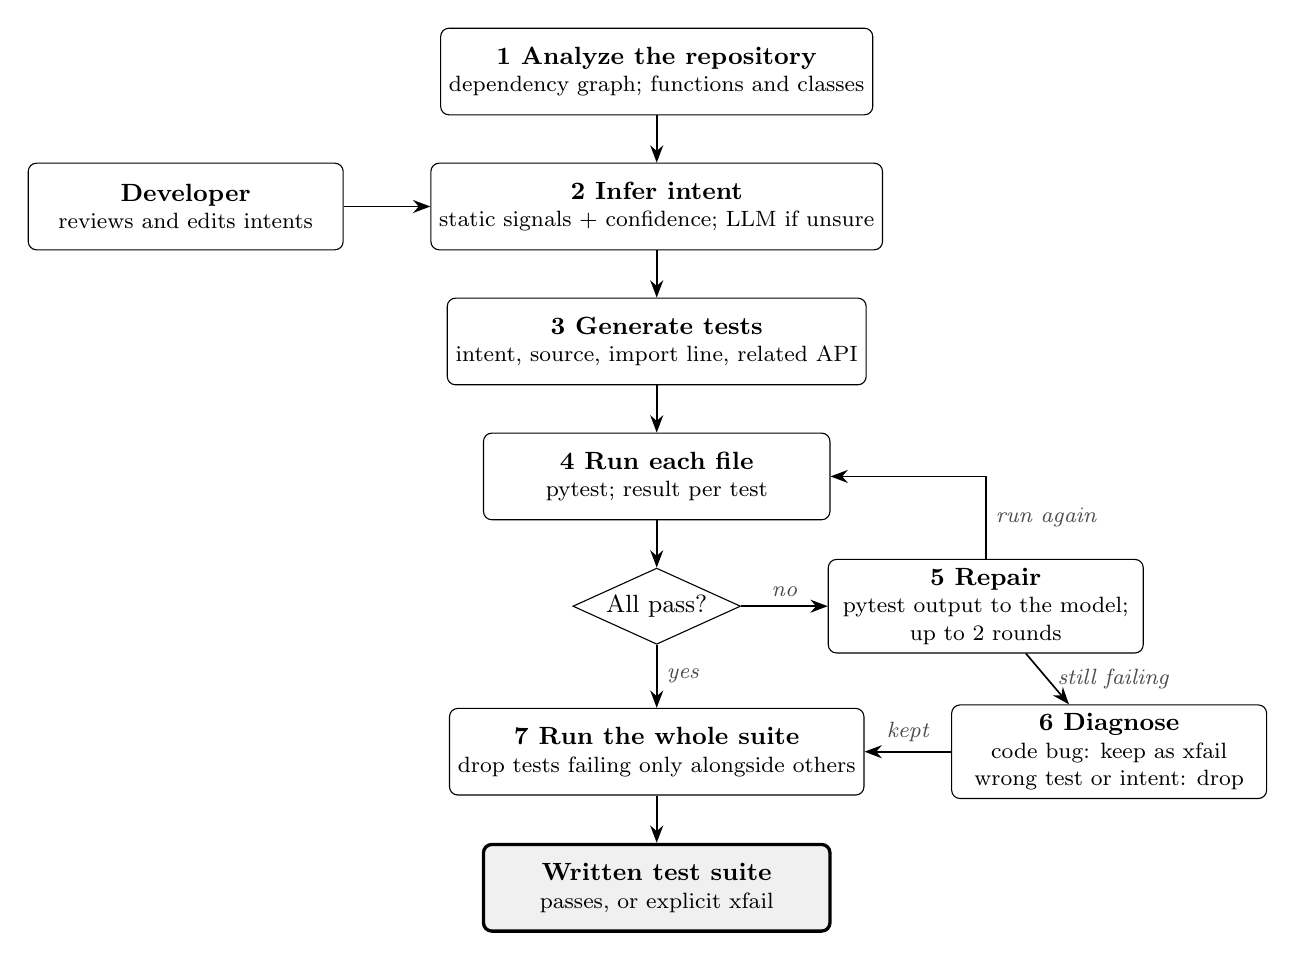
\begin{tikzpicture}[
  font=\small,
  node distance=6mm and 11mm,
  stage/.style={draw, rounded corners=3pt, align=center, minimum width=44mm, minimum height=11mm, inner sep=3pt},
  side/.style={draw, rounded corners=3pt, align=center, minimum width=40mm, minimum height=11mm, inner sep=3pt},
  final/.style={stage, very thick, fill=black!6},
  decision/.style={draw, diamond, aspect=2.2, align=center, inner sep=1pt},
  flow/.style={-{Stealth[length=2.2mm]}, semithick},
  note/.style={font=\footnotesize\itshape, text=black!70},
]
  \node[stage] (analyze) {\textbf{1 Analyze the repository}\\[-1pt]\footnotesize dependency graph; functions and classes};
  \node[stage, below=of analyze] (intent) {\textbf{2 Infer intent}\\[-1pt]\footnotesize static signals + confidence; LLM if unsure};
  \node[stage, below=of intent] (generate) {\textbf{3 Generate tests}\\[-1pt]\footnotesize intent, source, import line, related API};
  \node[stage, below=of generate] (run) {\textbf{4 Run each file}\\[-1pt]\footnotesize pytest; result per test};
  \node[decision, below=of run] (pass) {All pass?};
  \node[stage, below=8mm of pass] (suite) {\textbf{7 Run the whole suite}\\[-1pt]\footnotesize drop tests failing only alongside others};
  \node[final, below=of suite] (written) {\textbf{Written test suite}\\[-1pt]\footnotesize passes, or explicit xfail};

  \node[side, right=of pass] (repair) {\textbf{5 Repair}\\[-1pt]\footnotesize pytest output to the model;\\[-1pt]\footnotesize up to 2 rounds};
  \node[side, right=of suite] (diagnose) {\textbf{6 Diagnose}\\[-1pt]\footnotesize code bug: keep as xfail\\[-1pt]\footnotesize wrong test or intent: drop};
  \node[side, left=of intent] (dev) {\textbf{Developer}\\[-1pt]\footnotesize reviews and edits intents};

  \draw[flow] (analyze) -- (intent);
  \draw[flow] (intent) -- (generate);
  \draw[flow] (generate) -- (run);
  \draw[flow] (run) -- (pass);
  \draw[flow] (pass) -- node[note, right] {yes} (suite);
  \draw[flow] (suite) -- (written);
  \draw[flow] (pass) -- node[note, above] {no} (repair);
  \draw[flow] (repair.north) |- node[note, pos=0.25, right] {run again} (run.east);
  \draw[flow] (repair) -- node[note, right] {still failing} (diagnose);
  \draw[flow] (diagnose) -- node[note, above] {kept} (suite);
  \draw[flow] (dev) -- (intent);
\end{tikzpicture}

\caption{The \toolname{} pipeline. Every component follows the main column; failing tests enter the repair loop and, if repair fails, the diagnosis branch.}
\label{fig:pipeline}
\end{figure}

\subsection{Intent inference}
Static analysis scores each component $c$ from signals in its source:
\begin{equation}
\mathit{conf}(c) = \min\bigl(0.99, \max\bigl(0.1,\; 0.5 + w_{\mathrm{doc}} + w_{\mathrm{type}} + w_{\mathrm{name}} + w_{\mathrm{call}} - p_{\mathrm{cx}}\bigr)\bigr).
\end{equation}
Here $w_{\mathrm{doc}} \le 0.30$ grows with docstring length, $w_{\mathrm{type}} = 0.20$ if the signature has type hints, and $w_{\mathrm{name}} = 0.15$ for a recognized naming convention such as \code{validate\_*} or \code{is\_*}.
The call-site weight $w_{\mathrm{call}} \le 0.20$ grows with the number of call sites, and $p_{\mathrm{cx}} \le 0.15$ penalizes cyclomatic complexity above 5.
The intent text starts from the docstring's first sentence.
Below a threshold (default 0.6), an LLM re-infers the intent from the source and the more confident result is kept.
Intents are stored in SQLite.
A developer can review and edit them; an edited intent receives confidence 0.95 and is never replaced by a later run.

\subsection{Context and generation}
The test agent's prompt contains:
\begin{itemize}
  \item the intent and its confidence;
  \item the exact import line for the component;
  \item the imports at the top of its module, with relative imports made absolute;
  \item the bodiless public API (signatures, constructors, public methods) of the component's module and of the project modules it imports;
  \item up to 16{,}000 characters of the component's source.
\end{itemize}
The prompt asks the model to trace each expected value through the source, and to assert a property (type, length, membership, an exception) when an exact value is uncertain.
It also asks the model to build objects exactly as their signatures require, to put any file the code creates under pytest's \code{tmp\_path}, and never to mock the unit under test.
The model returns test functions, imports and fixtures as typed structured output, and each component gets its own test file.

\subsection{Execution and repair}
Each file runs alone under pytest in a subprocess.
The working directory is a throwaway temporary directory, with \code{--rootdir} at the repository, so tests that write relative paths cannot touch the user's files.
Results come from pytest's JUnit XML report and are matched to the test functions each generated test defines.
An error that prevents collection, such as a bad import or a syntax error, counts against every test in the file.
Failing tests go back to the model with their real pytest output, the fixtures and the related API, for up to two rounds.

\subsection{Diagnosis and the expected-failure policy}
Tests that still fail are classified against the stored intent:
\begin{itemize}
  \item \textbf{Wrong test} (\code{TEST\_WRONG}): the test misreads the intent.
  Errors raised by the test itself (import, syntax and name errors) always fall in this class.
  \item \textbf{Code bug} (\code{CODE\_BUG}): the code contradicts the intent.
  \item \textbf{Wrong intent} (\code{INTENT\_WRONG}): the inferred intent does not describe the code's purpose.
\end{itemize}
A suspected code bug is kept, decorated as in Listing~\ref{lst:xfail}.
Everything else is dropped, and a file that cannot be collected is never kept, because \code{xfail} cannot cover an error at import time.

\begin{lstlisting}[caption={A test \toolname{} kept as an expected failure, from the second run of inflection with M3 (Section~\ref{sec:second}). The reason is abbreviated.},label={lst:xfail},float=t]
@pytest.mark.xfail(reason='code2test: possible bug - The stated intent '
    'is "Return the singular form of a word, the reverse of pluralize." '
    'The singular of "campuses" is unambiguously "campus" ...', strict=False)
def test_singularize_campuses_to_campus():
    assert singularize("campuses") == "campus"
\end{lstlisting}

\subsection{Whole-suite check}
Tests that pass alone can fail together, for example when one test changes module-level state that another reads.
After per-file verification, all generated files run together, and tests that fail only there are dropped, for up to three rounds.

\subsection{Self-evaluation}\label{sec:benchmark}
Every run records how many components got passing tests and what share of the generated tests passed before any repair.
Skipped tests do not count as passing.
The \code{benchmark} command adds two measurements on the generated suite.

\paragraph{Mutation score.}
The benchmark enumerates single-site mutants in the tested components: flipped comparisons, swapped arithmetic and Boolean operators, changed constants, and \code{return None}.
Docstrings and type annotations are excluded, because no test can observe them.
It samples up to $N$ mutants and runs the \emph{whole} generated suite against each one.
It also reports the share killed by the mutated component's own tests.
Before mutating a file it keeps a byte-exact backup, and it restores the file on exit, including on SIGTERM; a run that was killed is repaired the next time the command starts.

\paragraph{Diagnosis accuracy.}
Failures with a known cause are passed to the diagnosis agent.
\begin{itemize}
  \item A test of the mutated component that fails on a mutant is a \code{CODE\_BUG} case.
  The mutated line must lie within the source the agent is shown.
  \item A passing test whose first literal expected value is perturbed is a \code{TEST\_WRONG} case (an integer is incremented, or a string loses its last character).
  It counts only if the perturbed assertion is what fails.
\end{itemize}
The perturbations deliberately leave no marker in the code, such as a ``\_wrong'' suffix, that would give the answer away.

% -------------------------------------------------------------------------
\section{Implementation}
% -------------------------------------------------------------------------

\toolname{} is a Python~3.12 command-line tool (\code{test}, \code{verify}, \code{intent}, \code{benchmark}, \code{report}).
Its dependency analysis comes from the CodeWiki analyzer (tree-sitter, several languages); only Python components get tests in the current version.
The three agents use pydantic-ai with typed structured output and up to three output retries.
They work with any model pydantic-ai supports, including OpenAI-compatible endpoints.
HTTP 401, 403 and 404 responses stop the run, so a bad key or model name cannot produce an apparently successful run with no tests.
The tool's own test suite (over 100 tests) drives the whole pipeline offline with scripted models.

% -------------------------------------------------------------------------
\section{Evaluation}\label{sec:evaluation}
% -------------------------------------------------------------------------

We answer four research questions.
\begin{description}[leftmargin=1.2cm,style=nextline]
  \item[RQ1] How many components end up with passing tests, and how many generated tests pass before any repair?
  \item[RQ2] Do the written suites detect injected faults?
  \item[RQ3] How accurate is the failure diagnosis on failures with a known cause?
  \item[RQ4] What breaks when scripted test doubles are replaced by a real model?
\end{description}

\subsection{Setup}
\paragraph{Subjects.}
We used two pure-Python libraries from PyPI, after removing each library's own tests:
\begin{itemize}
  \item \textbf{inflection 0.5.1}: 426 lines and 13 components; string functions over module-level rule tables.
  \item \textbf{TinyDB 4.8.2}: 2{,}170 lines and 26 components; classes with state, JSON file storage, caching middleware and a query language.
\end{itemize}

\paragraph{Models.}
MiniMax \code{MiniMax-M3.1-Flash-Preview} (``Flash'') and \code{MiniMax-M3} (``M3''), accessed through MiniMax's OpenAI-compatible API with default settings.

\paragraph{Procedure.}
For each subject and model, one run of \code{code2test test --auto}, then \code{code2test verify}, then \code{code2test benchmark} with 80 sampled mutants and 15 diagnosis cases per expected cause.
These first runs are the main results.
A second run of each configuration, made later, shows how much the results vary (Section~\ref{sec:second}).
The MVP targets come from the project proposal: at least 70\% of components with tests, at least 80\% of tests passing before repair, and at least 75\% diagnosis accuracy.

\begin{table}[t]
\centering
\small
\caption{Results per subject and model (first runs). Test cases count parametrized cases separately. Mutants are sampled from the components that have tests, so the two TinyDB runs use different samples.}
\label{tab:results}
\begin{tabular}{@{}l rr rr@{}}
\toprule
& \multicolumn{2}{c}{inflection} & \multicolumn{2}{c}{TinyDB} \\
\cmidrule(lr){2-3}\cmidrule(lr){4-5}
Measure & Flash & M3 & Flash & M3 \\
\midrule
Components with passing tests & \InflectionFlashWithTests/\InflectionFlashComponents & \InflectionMThreeWithTests/\InflectionMThreeComponents & \TinyDBFlashWithTests/\TinyDBFlashComponents & \TinyDBMThreeWithTests/\TinyDBMThreeComponents \\
\quad acceptance rate (target 70\%) & \InflectionFlashAcceptance & \InflectionMThreeAcceptance & \TinyDBFlashAcceptance & \TinyDBMThreeAcceptance \\
Tests generated & \InflectionFlashGenerated & \InflectionMThreeGenerated & \TinyDBFlashGenerated & \TinyDBMThreeGenerated \\
\quad passing before repair (target 80\%) & \InflectionFlashFirstRate & \InflectionMThreeFirstRate & \TinyDBFlashFirstRate & \TinyDBMThreeFirstRate \\
Tests kept / dropped & \InflectionFlashKept/\InflectionFlashDropped & \InflectionMThreeKept/\InflectionMThreeDropped & \TinyDBFlashKept/\TinyDBFlashDropped & \TinyDBMThreeKept/\TinyDBMThreeDropped \\
Tests kept as xfail & \InflectionFlashXfail & \InflectionMThreeXfail & \TinyDBFlashXfail & \TinyDBMThreeXfail \\
Repair rounds & \InflectionFlashRepairs & \InflectionMThreeRepairs & \TinyDBFlashRepairs & \TinyDBMThreeRepairs \\
Test cases passing in \code{verify} & \InflectionFlashCasesPassed/\InflectionFlashCasesTotal & \InflectionMThreeCasesPassed/\InflectionMThreeCasesTotal & \TinyDBFlashCasesPassed/\TinyDBFlashCasesTotal & \TinyDBMThreeCasesPassed/\TinyDBMThreeCasesTotal \\
Time to generate and repair (s) & \InflectionFlashSeconds & \InflectionMThreeSeconds & \TinyDBFlashSeconds & \TinyDBMThreeSeconds \\
\midrule
Mutants killed, whole suite & \InflectionFlashKilled/\InflectionFlashMutants & \InflectionMThreeKilled/\InflectionMThreeMutants & \TinyDBFlashKilled/\TinyDBFlashMutants & \TinyDBMThreeKilled/\TinyDBMThreeMutants \\
\quad mutation score & \InflectionFlashMutationScore & \InflectionMThreeMutationScore & \TinyDBFlashMutationScore & \TinyDBMThreeMutationScore \\
\quad by the component's own tests & \InflectionFlashOwnScore & \InflectionMThreeOwnScore & \TinyDBFlashOwnScore & \TinyDBMThreeOwnScore \\
\midrule
Diagnosis correct (target 75\%) & \InflectionFlashDiagAccuracy & \InflectionMThreeDiagAccuracy & \TinyDBFlashDiagAccuracy & \TinyDBMThreeDiagAccuracy \\
\quad code-bug cases & \InflectionFlashCodeBugCorrect/\InflectionFlashCodeBugCases & \InflectionMThreeCodeBugCorrect/\InflectionMThreeCodeBugCases & \TinyDBFlashCodeBugCorrect/\TinyDBFlashCodeBugCases & \TinyDBMThreeCodeBugCorrect/\TinyDBMThreeCodeBugCases \\
\quad wrong-test cases & \InflectionFlashTestWrongCorrect/\InflectionFlashTestWrongCases & \InflectionMThreeTestWrongCorrect/\InflectionMThreeTestWrongCases & \TinyDBFlashTestWrongCorrect/\TinyDBFlashTestWrongCases & \TinyDBMThreeTestWrongCorrect/\TinyDBMThreeTestWrongCases \\
\bottomrule
\end{tabular}
\end{table}

\subsection{RQ1: Acceptance and first-run validity}
Table~\ref{tab:results} shows that every run met both generation targets.
Each written suite passed \code{verify}; the one TinyDB case not counted as passing was skipped by its own test, not failed.
The single TinyDB component without tests differed by model.
With Flash, the generation call for \code{LRUCache} failed after its retries.
With M3, the model wrote a single test for the \code{TinyDB} class.
That test still failed after two repair rounds, was diagnosed as a wrong test, and was dropped.

The stronger model did not dominate.
M3 passed more tests before repair than Flash on TinyDB (\TinyDBMThreeFirstRate{} vs.\ \TinyDBFlashFirstRate) but fewer on inflection (\InflectionMThreeFirstRate{} vs.\ \InflectionFlashFirstRate).
It also wrote fewer tests in every case.

No test was kept as an expected failure in any first run, and every diagnosis made during generation was a wrong test.
On two mature libraries this is the desired outcome: the expected-failure path never accused correct code.
The one test kept as an expected failure across all runs came from a second run and exposes a real defect (Section~\ref{sec:second}).

\paragraph{Where the intents came from.}
Both libraries document nearly every component.
No inflection component and \TinyDBFlashIntentsBelow{} of the 26 TinyDB components scored below the 0.6 threshold, so the model re-inferred \TinyDBFlashIntentsFromModel{} intents per TinyDB run and none for inflection.
Every other intent came from static signals, almost always the docstring's first sentence.
On these subjects the intent stage therefore added little beyond the docstring, and the results do not isolate its effect.

\subsection{RQ2: Fault detection}
On whole-suite mutation analysis, the suites killed between \MinMutationScore{} and \MaxMutationScore{} of the sampled mutants (Table~\ref{tab:results}).
Tests of other components added few kills: the whole suite killed \InflectionFlashKilled{}, \InflectionMThreeKilled{}, \TinyDBFlashKilled{} and \TinyDBMThreeKilled{} mutants, against \InflectionFlashKilledOwn{}, \InflectionMThreeKilledOwn{}, \TinyDBFlashKilledOwn{} and \TinyDBMThreeKilledOwn{} for the mutated component's own tests.
The survivors are concentrated rather than spread out.

\paragraph{inflection.}
\InflectionFlashTopMutants{} of the 80 sampled mutants fall in \code{\_irregular}, which builds the rules for irregular words such as \emph{person}/\emph{people} and \emph{cow}/\emph{kine} when the module is imported.
Flash wrote a single test for it, which checks how many rules are inserted, and no Flash test checks an irregular word through \code{pluralize} or \code{singularize}.
That suite killed \InflectionFlashTopKilled{} of the \InflectionFlashTopMutants{} \code{\_irregular} mutants.
M3 wrote 19 tests for \code{\_irregular} that check words whose singular and plural share a first letter, such as \emph{person}/\emph{people}.
It killed \InflectionMThreeTopKilled{}; its survivors are in the branch for words whose first letters differ, such as \emph{cow}/\emph{kine}.
Outside \code{\_irregular}, the suites killed \InflectionFlashRestKilled{} of \InflectionFlashRestMutants{} (Flash) and \InflectionMThreeRestKilled{} of \InflectionMThreeRestMutants{} (M3) mutants.
Passing tests can thus check structure rather than behavior, and whether a run tests a behavior at all varies between runs (Section~\ref{sec:threats}).

\paragraph{TinyDB.}
\TinyDBFlashStringSurvivors{} of \TinyDBFlashSurvivors{} (Flash) and \TinyDBMThreeStringSurvivors{} of \TinyDBMThreeSurvivors{} (M3) surviving mutants change a string literal.
These are the operator names that \code{Query} uses as hash keys, exception messages and \code{repr} text.
Tests that check an exception's type but not its message cannot see such changes, and many hash-key changes are likely equivalent mutants, because a key only needs to differ from the others.

\subsection{RQ3: Diagnosis accuracy}
On failures of known cause, the diagnosis agent was correct in \InflectionFlashDiagAccuracy{}, \InflectionMThreeDiagAccuracy{}, \TinyDBFlashDiagAccuracy{} and \TinyDBMThreeDiagAccuracy{} of cases across the four runs, above the 75\% target.
It made one error across the four runs.
In inflection with Flash, a mutant sent \code{\_irregular} down its other branch, so the test's expected rule counts no longer held.
The agent read the mutated source and judged the test wrong, because the code now inserted more rules than the test expected.
The intent (``a convenience function to add appropriate rules to plurals and singular for irregular words'') says nothing about the number of rules, so the agent sided with the code.
This is the misguidance effect~\cite{zhao2026misguidance} in miniature: where the intent is silent, the code decides.
The cases are synthetic, and the threats below explain why they are likely easier than real failures.

\subsection{Second runs and a real defect}\label{sec:second}
We ran each configuration a second time, later and with the same pipeline.\footnote{The second runs used a later version of \toolname{} that removed code inherited from CodeWiki which the pipeline does not use. Under that version, the first runs' suites reproduced their verification and mutation results exactly.}
Table~\ref{tab:second} compares the two runs.
Every second run met the three targets again.
The share of tests passing before repair varied most: on inflection it fell from \InflectionFlashFirstRate{} to \InflectionFlashSecondFirstRate{} with Flash and rose from \InflectionMThreeFirstRate{} to \InflectionMThreeSecondFirstRate{} with M3.
The largest change in mutation score was on TinyDB with Flash, from \TinyDBFlashMutationScore{} to \TinyDBFlashSecondMutationScore.
The second runs' two diagnosis errors were of the same kind as the first runs' one: failures caused by a mutant, judged to be wrong tests because the agent sided with the mutated code.
Generation times are not compared, because the second runs shared the machine with other jobs.

\begin{table}[t]
\centering
\small
\caption{First and second run of each configuration (first / second).}
\label{tab:second}
\begin{tabular}{@{}l cccc@{}}
\toprule
& \multicolumn{2}{c}{inflection} & \multicolumn{2}{c}{TinyDB} \\
\cmidrule(lr){2-3}\cmidrule(lr){4-5}
Measure & Flash & M3 & Flash & M3 \\
\midrule
Acceptance rate & \InflectionFlashAcceptance{} / \InflectionFlashSecondAcceptance & \InflectionMThreeAcceptance{} / \InflectionMThreeSecondAcceptance & \TinyDBFlashAcceptance{} / \TinyDBFlashSecondAcceptance & \TinyDBMThreeAcceptance{} / \TinyDBMThreeSecondAcceptance \\
Passing before repair & \InflectionFlashFirstRate{} / \InflectionFlashSecondFirstRate & \InflectionMThreeFirstRate{} / \InflectionMThreeSecondFirstRate & \TinyDBFlashFirstRate{} / \TinyDBFlashSecondFirstRate & \TinyDBMThreeFirstRate{} / \TinyDBMThreeSecondFirstRate \\
Tests generated & \InflectionFlashGenerated{} / \InflectionFlashSecondGenerated & \InflectionMThreeGenerated{} / \InflectionMThreeSecondGenerated & \TinyDBFlashGenerated{} / \TinyDBFlashSecondGenerated & \TinyDBMThreeGenerated{} / \TinyDBMThreeSecondGenerated \\
Tests kept as xfail & \InflectionFlashXfail{} / \InflectionFlashSecondXfail & \InflectionMThreeXfail{} / \InflectionMThreeSecondXfail & \TinyDBFlashXfail{} / \TinyDBFlashSecondXfail & \TinyDBMThreeXfail{} / \TinyDBMThreeSecondXfail \\
Mutation score & \InflectionFlashMutationScore{} / \InflectionFlashSecondMutationScore & \InflectionMThreeMutationScore{} / \InflectionMThreeSecondMutationScore & \TinyDBFlashMutationScore{} / \TinyDBFlashSecondMutationScore & \TinyDBMThreeMutationScore{} / \TinyDBMThreeSecondMutationScore \\
Diagnosis correct & \InflectionFlashDiagAccuracy{} / \InflectionFlashSecondDiagAccuracy & \InflectionMThreeDiagAccuracy{} / \InflectionMThreeSecondDiagAccuracy & \TinyDBFlashDiagAccuracy{} / \TinyDBFlashSecondDiagAccuracy & \TinyDBMThreeDiagAccuracy{} / \TinyDBMThreeSecondDiagAccuracy \\
\bottomrule
\end{tabular}
\end{table}

\paragraph{A real defect in inflection.}
In the second run of inflection with M3, one test still failed after repair, was diagnosed as a code bug, and was kept as an expected failure (Listing~\ref{lst:xfail}).
The test is right.
inflection 0.5.1 singularizes \emph{campuses} to \emph{campuse} and \emph{campus} to \emph{campu}, and pluralizes \emph{campus} to \emph{campus}.
Its rule list has entries for \emph{bus}, \emph{alias} and \emph{status}; other words ending in \emph{-us} fall through to catch-all rules that drop or keep a final \emph{s}, so \emph{viruses}, \emph{bonuses} and \emph{censuses} fail the same way.
Neither inflection's own test suite nor any other generated suite in our runs tests these words.
The model's explanation names a rule for \emph{campus} that the library does not have, but its verdict is correct.
A generator that keeps only passing tests would have dropped this test or rewritten it to expect \emph{campuse}.

This is one case in eight runs, on a word the model happened to choose.
It shows the expected-failure path working on real code; it does not show that intent-first generation avoids locking in bugs in general (Section~\ref{sec:discussion}).

\subsection{RQ4: What a real model broke}\label{sec:failures}
During development, the tool's own tests used scripted models and passed throughout.
The first real-model runs exposed the eight failure modes in Table~\ref{tab:failures}.
Each was fixed with a regression test before the results above were measured.
On inflection the written suite went from failing to collect in the first real-model run during development, to 676 of 680 test cases passing in the next, to passing in full from the third on.

\begin{table}[t]
\centering
\small
\caption{Failure modes found only with a real model, and their fixes.}
\label{tab:failures}
\begin{tabularx}{\linewidth}{@{}L L L@{}}
\toprule
Failure mode & Symptom & Fix \\
\midrule
Rejected API key looked like success & Every call returned HTTP 401, yet the run exited 0 with no tests & Authentication and unknown-model errors stop the run \\
Nested functions treated as components & inflection's \code{caseinsensitive} lives inside \code{\_irregular}; its tests could never import it & Skip functions nested in functions \\
Unimportable files kept as xfail & xfail cannot cover a module-level import error; the whole suite failed to collect & Never keep a file that cannot be collected; errors raised by the test count as a wrong test \\
Reported test names differ from defined names & Failures matched no test, so failing files were kept unverified & Match results on the functions each test defines \\
Doubly escaped code & Literal \textbackslash n and \textbackslash" in code or fixtures broke whole files & Unescape only when that makes the code compile \\
Tests interfering across files & Tests registering irregular words broke \code{pluralize} tests in the combined run & Whole-suite check after per-file verification \\
Missing API context & Tests passed an instance where TinyDB expects a storage class; 0 of 6 passed & Related project API in the prompt; 43 of 43 passed \\
Tests writing into the repository & An unrepaired test created \code{some/path} in the project directory & Run pytest from a temporary directory; prompt requires \code{tmp\_path} \\
\bottomrule
\end{tabularx}
\end{table}

% -------------------------------------------------------------------------
\section{Discussion}\label{sec:discussion}
% -------------------------------------------------------------------------

\subsection{What is new}
Table~\ref{tab:novelty} states, claim by claim, what has a precedent.
None of \toolname{}'s techniques is new on its own.
The closest system, TestAgent~\cite{zhang2026testagent}, shares the stored summary, the bug-versus-test triage and the retention of defect-revealing tests, and it was evaluated on larger Java and Python projects.
What \toolname{} adds is a specific combination:
\begin{itemize}
  \item an intent that is scored and developer-editable, and reused across runs and in triage;
  \item a third diagnosis class for a wrong intent;
  \item retention of suspected bugs as expected failures, so the delivered suite stays green;
  \item self-evaluation, including triage accuracy, on the user's own project.
\end{itemize}
We therefore present \toolname{} as a tool and experience report rather than a new technique.

\begin{table}[t]
\centering
\small
\caption{Novelty of each claim, judged against the closest prior work.}
\label{tab:novelty}
\begin{tabularx}{\linewidth}{@{}L L l@{}}
\toprule
Claim & Closest prior work & Verdict \\
\midrule
Infer intent before writing tests & ChatTester, Test4Py, TestAgent, IGTG\&R, Zhao et al. & Incremental \\
Classify failures as test, code or intent & TestAgent, Testora, JiTTests & Incremental \\
Keep bug-revealing tests in the suite & TestAgent (as failing tests) & Incremental \\
Repair, discard, cross-test interference & CoverUp, TestGen-LLM & Not new \\
Bodiless API context & CoverUp & Not new \\
Dependency-ordered summaries & Test4Py & Not new \\
Triage accuracy from failures of known cause & Konstantinou et al. & Not new as a method \\
Real-model failure modes; two-model comparison & -- & Empirical \\
\bottomrule
\end{tabularx}
\end{table}

\subsection{The open question}
The design is motivated by the misguidance effect~\cite{mathews2024design,zhao2026misguidance}, but this paper does not yet show that \toolname{} avoids it.
Both subjects are mature, and the study was not designed around known bugs; the one defect it found (Section~\ref{sec:second}) came up by chance.
The decisive experiment uses buggy programs with known fixes, such as Refactory as in Mathews and Nagappan, and BugsInPy, and compares \toolname{} with CoverUp, Cover-Agent and TestAgent under the same model.
For each tool it would count tests that pass on the buggy version and fail on the fix (bugs locked in) against tests that flag the bug, with and without intent-first generation.
That study is the natural next step.

\subsection{Threats to validity}\label{sec:threats}
\begin{itemize}
  \item \textbf{Scale and variance.} Two small libraries and two runs per configuration, which shows that results vary (Table~\ref{tab:second}) but does not estimate by how much. The variance we saw during development was larger.
  In a development run with Flash and an earlier version of the tool, the inflection suite had 33 tests for \code{\_irregular}, several checking irregular words through \code{pluralize} and \code{singularize}, and killed all 80 mutants of its own sample even when only each component's own tests ran.
  Across development runs, TinyDB's mutation score with Flash ranged from 64\% to 79\% under that per-component scoring.
  \item \textbf{Mutants.} The 80 mutants are sampled uniformly from all mutation sites, so large functions dominate the sample: half of inflection's sample falls in \code{\_irregular}. There is no filter for equivalent mutants.
  \item \textbf{Synthetic triage labels.} Mutated code is a code bug by construction, and the intent was inferred from the original code. Wrong-test cases differ from a passing test by one perturbed literal. Both make the cases easier to classify than real failures.
  \item \textbf{Training data.} Both libraries are public and may appear in the models' training data.
  \item \textbf{Same authors.} The tool and the benchmark come from the same authors. An early benchmark version left markers in its injected faults that overstated diagnosis accuracy until it was fixed. Two metric definitions were also corrected during development: skipped tests no longer count as passing, and re-runs no longer report 0\% acceptance. All reported numbers use the corrected definitions.
\end{itemize}

\subsection{Limitations}
Only Python components get tests.
An expected-failure test is only as good as the diagnosis behind it: a wrong code-bug verdict keeps a wrong test as an expected failure.
Code that needs databases, networks or other services gets tests only when the model can build fixtures for it.
Each run sends source code to the model provider and costs one or more model calls per component.

% -------------------------------------------------------------------------
\section{Conclusion}
% -------------------------------------------------------------------------

\toolname{} infers and stores an explicit intent for each component of a legacy Python codebase.
It then generates, executes, repairs and diagnoses tests against that intent, and keeps suspected bugs visible as expected failures rather than filtering them out.
On two libraries and two models it produced passing tests for nearly every component, and in the first runs at least \MinFirstRate{} of generated tests passed before any repair.
The suites killed \MinMutationScore--\MaxMutationScore{} of sampled mutants; most survivors sat in behavior a run had tested only structurally, or changed strings that tests do not observe.
The diagnosis was correct on all but one of the first runs' failures of known cause.
In a second run, \toolname{} kept a test as an expected failure that exposes a real defect in inflection, where a filter for passing tests would have discarded it.
Its techniques have precedents; its value lies in the combination, the built-in self-evaluation, and the failure modes we document.
Whether intent-first generation avoids locking bugs into generated suites is the question we plan to answer next.

\section*{Data Availability}
The tool, the experiment scripts and all raw results are available at \url{https://github.com/Cirkitly/code2test}, under \code{research/}.
For each run, first and second, the results include the generated test suite, the inferred intents, the run metrics, the benchmark output with every surviving mutant and diagnosis case, and the verification log.
\code{research/scripts/run\_experiments.sh} reproduces the runs, given a MiniMax API key.

\bibliographystyle{plainnat}
\bibliography{references}

\end{document}
